\chapter{Arhitectura Aplicației}
\label{chap:ch4}

\section{Prezentare Generală}

Aplicația este structurată ca un sistem modular de procesare video în timp real, cu scopul de a detecta planul solului și de a planifica o traiectorie navigabilă pe baza unei hărți de adâncime generate de un model de învățare profundă. Sistemul suportă două profiluri hardware distincte: un host cu GPU NVIDIA, folosind PyTorch și CUDA pentru inferență, respectiv un Raspberry Pi 5 cu accelerator NPU Hailo-8, folosind biblioteca \texttt{hailort}. Indiferent de profilul activ, restul pipeline-ului rămâne identic, ceea ce face posibilă portabilitatea codului fără modificări.

Întreaga bază de cod este scrisă în Python 3.11+ și organizată în două mari componente: un \textbf{backend} de procesare și o \textbf{interfață grafică} (GUI) construită cu PyQt6. Separarea clară dintre aceste două componente permite înlocuirea sau testarea fiecăreia independent.

\section{Principii de Proiectare Utilizate}

\subsection{Separarea Responsabilităților}

Fiecare modul al aplicației are o singură responsabilitate bine definită. Modulul \texttt{config.py} se ocupă exclusiv de citirea și validarea configurației. Modulul \texttt{hardware.py} abstractizează diferențele dintre platformele hardware. Modulul \texttt{ground.py} conține exclusiv logica de detectare a planului solului, fără nicio referință la interfața grafică sau la camera video. Această separare face ca fiecare componentă să poată fi testată, înlocuită sau extinsă fără a afecta restul sistemului.

\subsection{Programare Orientată pe Obiecte}

Clasele sunt folosite acolo unde există stare internă care trebuie gestionată pe durata vieții unui obiect. \texttt{HardwareProfile} encapsulează profilul hardware activ și expune proprietăți derivate (\texttt{is\_nvidia}, \texttt{is\_rpi}, \texttt{is\_metric}) fără a expune câmpurile interne. \texttt{CalibrationService} grupează operațiile de calibrare împreună cu configurația de care au nevoie. \texttt{DepthPipeline} gestionează întregul ciclu de viață al procesării unui cadru video: deschiderea camerei, încărcarea modelului, firul de captură, și eliberarea resurselor la oprire. \texttt{ModelRegistry} abstractizează alegerea backend-ului de inferență, astfel că apelantul nu știe și nu trebuie să știe dacă inferența rulează pe CUDA sau pe NPU Hailo.

Funcțiile pure sunt preferate claselor atunci când nu există stare internă de gestionat. Modulele \texttt{ground.py}, \texttt{path.py} și \texttt{visualization.py} sunt compuse exclusiv din funcții, deoarece transformările pe care le realizează (proiecție 3D, RANSAC, A*, suprapunere vizuală) sunt fără efecte secundare și nu necesită obiecte.

\subsection{Configurație Tipizată}

Configurația aplicației este citită o singură dată la pornire din fișierul \texttt{config.toml} și transformată într-un arbore de \texttt{dataclass}-uri imutabile (\texttt{frozen=True}): \texttt{AppConfig}, \texttt{CameraConfig}, \texttt{CalibrationConfig}, \texttt{GroundConfig} etc. Această abordare elimină accesul prin chei de tip șir de caractere (de exemplu \texttt{cfg["ground"]["seed\_region"]}) și înlocuiește șirul de caractere cu atribute tipizate (\texttt{cfg.ground.seed\_region}), ceea ce permite detectarea erorilor de configurare la încărcare, nu la rulare, și oferă autocompletare în mediile de dezvoltare.

\subsection{Comunicare Asincronă prin Semnale Qt}

Inferența modelului de adâncime și captura video rulează în fire de execuție separate față de firul principal al interfeței grafice. Comunicarea dintre fire se realizează exclusiv prin mecanismul de semnale și sloturi al Qt (\texttt{pyqtSignal}), care garantează că actualizările interfeței grafice au loc întotdeauna pe firul principal. Această abordare previne blocarea interfeței în timpul procesării și elimina condițiile de cursă (\textit{race conditions}) specifice accesului concurent la widget-uri.

\subsection{Inversiunea Dependențelor la Nivel de Backend}

Modulul \texttt{model.py} acționează ca un registru de factory: în funcție de profilul hardware activ, deleghează apelurile fie către \texttt{model\_nvidia.py}, fie către \texttt{model\_rpi.py}. Pipeline-ul central (\texttt{pipeline.py}) depinde exclusiv de interfața abstractă a lui \texttt{ModelRegistry}, nu de implementările concrete. Adăugarea unui nou backend (de exemplu un alt accelerator hardware) necesită doar adăugarea unui fișier nou și a unui caz în registru, fără a modifica pipeline-ul sau GUI-ul.

\section{Arhitectura pe Straturi}

Aplicația este organizată în patru straturi distincte, cu dependențe strict direcționate de sus în jos. Stratul superior depinde de cel imediat inferior; niciun strat nu cunoaște existența straturilor superioare.

\subsection{Stratul de Prezentare (GUI)}

Corespunde pachetului \texttt{gui/} și este responsabil exclusiv de interacțiunea cu utilizatorul. Conține:
\begin{itemize}
    \item \texttt{app.py} — fereastra principală (\texttt{MainWindow}), care gestionează navigarea între ecrane printr-un \texttt{QStackedWidget};
    \item \texttt{main\_menu.py} — ecranul de pornire cu cele patru acțiuni principale;
    \item \texttt{calibration.py} — ecranul de calibrare, inclusiv dialogul modal cu previzualizare live și afișarea scorului RMS;
    \item \texttt{settings.py} — formularul de editare a configurației, cu scriere înapoi în \texttt{config.toml};
    \item \texttt{system\_view.py} — vizualizarea live a sistemului, cu bara laterală de opțiuni și redarea cadrelor procesate;
    \item \texttt{components.py} — widget-uri reutilizabile: \texttt{StyledButton}, \texttt{NavBar}, \texttt{ToggleSwitch}, \texttt{SectionHeader}, \texttt{StatusBadge};
    \item \texttt{styles.py} — paleta de culori, fonturile și foaia de stiluri globală Qt.
\end{itemize}

Stratul de prezentare nu realizează nicio procesare de imagine sau inferență. El pornește și oprește pipeline-ul prin metode publice și primește rezultate prin semnale Qt.

\subsection{Stratul de Orchestrare (Pipeline)}

Corespunde modulului \texttt{pipeline.py} și reprezintă punctul central de coordonare al aplicației. Clasa \texttt{DepthPipeline} gestionează:
\begin{itemize}
    \item un fir de captură dedicat, care citește continuu cadre de la cameră și păstrează întotdeauna cel mai recent cadru disponibil;
    \item un fir de inferență, care consumă cadrele, rulează pipeline-ul complet și emite rezultate prin semnale Qt;
    \item starea internă a sistemului: hărțile de corecție a distorsiunii, matricea intrinsecă activă, planul anterior detectat.
\end{itemize}

Rezultatul unui cadru procesat este reprezentat de dataclass-ul \texttt{FrameResult}, care agregă cadrul RGB, harta de adâncime, masca solului, traiectoria A*, punctele de start/stop și coeficienții planului.

\subsection{Stratul de Procesare (Core)}

Conține implementările algoritmice independente de hardware și de interfața grafică:
\begin{itemize}
    \item \texttt{ground.py} — detectarea planului solului prin RANSAC vectorizat cu eșantionare subpixelică, urmat de rafinare SVD și construirea măștii direct în spațiul 2D al imaginii;
    \item \texttt{path.py} — planificarea traiectoriei prin algoritmul A* cu conectivitate pe 8 direcții și euristică octilă admisibilă;
    \item \texttt{visualization.py} — suprapunerea vizuală a măștii solului, a traiectoriei și a barei de stare pe cadrul video;
    \item \texttt{camera.py} — deschiderea camerei (V4L2 sau picamera2), construirea hărților de corecție a distorsiunii și aplicarea lor;
    \item \texttt{calibration.py} — captarea pozelor de calibrare și rezolvarea matricei intrinseci prin \texttt{cv2.calibrateCamera}.
\end{itemize}

\subsection{Stratul de Infrastructură}

Conține modulele care nu realizează procesare propriu-zisă, ci furnizează configurație, abstractizare hardware și acces la modele:
\begin{itemize}
    \item \texttt{config.py} — citirea fișierului \texttt{config.toml} și construirea arborelui de \texttt{dataclass}-uri tipizate;
    \item \texttt{hardware.py} — \texttt{HardwareProfile}: abstractizarea profilului activ și selecția dispozitivului de calcul;
    \item \texttt{model.py} — \texttt{ModelRegistry}: factory care deleghează încărcarea și inferența modelului de adâncime;
    \item \texttt{model\_nvidia.py} — backend PyTorch + CUDA, folosind DepthAnything3 cu AMP și \texttt{torch.compile} opțional;
    \item \texttt{model\_rpi.py} — backend Hailo, folosind \texttt{hailort} pentru inferența pe NPU-ul Hailo-8;
    \item \texttt{main.py} — punctul de intrare în aplicație; lansează GUI-ul sau modul headless.
\end{itemize}

\section{Diagrama Straturilor}

\begin{figure}[htbp]
\centering
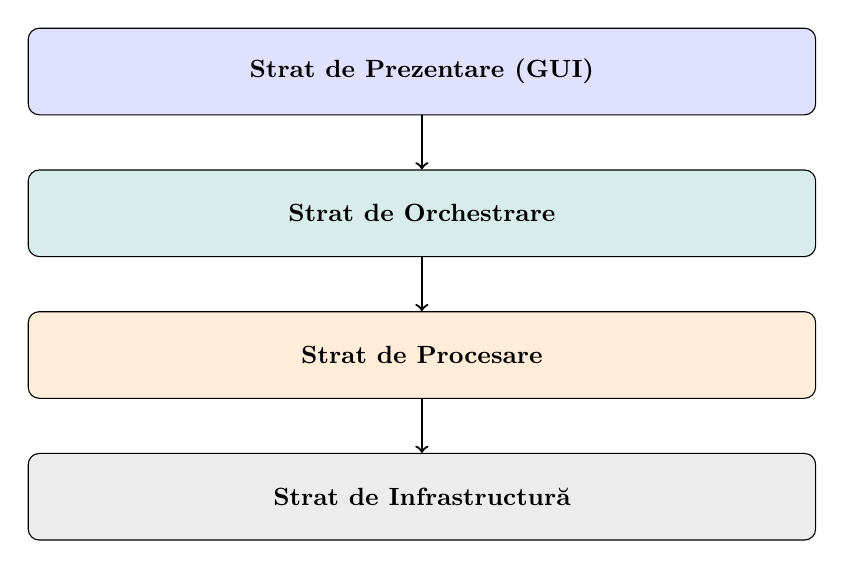
\begin{tikzpicture}[
    layer/.style={
        draw, rounded corners=4pt,
        minimum width=10cm, minimum height=1.1cm,
        align=center, font=\small\bfseries
    },
    sublabel/.style={font=\footnotesize, text=gray}
]

\node[layer, fill=blue!12]   (gui)      at (0, 0)    {Strat de Prezentare (GUI)};
\node[layer, fill=teal!15]   (pipeline) at (0, -1.8)  {Strat de Orchestrare};
\node[layer, fill=orange!15] (core)     at (0, -3.6)  {Strat de Procesare};
\node[layer, fill=gray!15]   (infra)    at (0, -5.4)  {Strat de Infrastructură};

\draw[->, thick] (gui.south)      -- (pipeline.north);
\draw[->, thick] (pipeline.south) -- (core.north);
\draw[->, thick] (core.south)     -- (infra.north);

\end{tikzpicture}
\caption{Arhitectura pe straturi a aplicației. Dependențele sunt direcționate exclusiv de sus în jos.}
\label{fig:layers}
\end{figure}

\section{Fluxul de Date}

La pornirea sistemului, \texttt{MainWindow} încarcă configurația tipizată din \texttt{config.toml} printr-un apel la \texttt{AppConfig.load()}. Când utilizatorul apasă butonul \textit{START} din ecranul de vizualizare live, \texttt{SystemViewWidget} instanțiază un \texttt{DepthPipeline} și pornește firul de inferență. Acesta inițializează \texttt{ModelRegistry} (care, în funcție de profilul hardware, încarcă fie modelul PyTorch, fie fișierul HEF pentru Hailo), deschide camera prin \texttt{CameraFactory} și pornește firul de captură.

La fiecare cadru disponibil, pipeline-ul aplică corecția de distorsiune, rulează inferența pentru a obține harta de adâncime, detectează planul solului prin RANSAC vectorizat și construiește masca, planifică traiectoria prin A*, și împachetează toate rezultatele într-un obiect \texttt{FrameResult}. Acesta este transmis stratului de prezentare prin semnalul Qt \texttt{\_result\_signal}, unde \texttt{SystemViewWidget} aplică suprapunerile vizuale și actualizează widget-ul de afișare.

Utilizatorul poate modifica parametrii sistemului în orice moment prin ecranul \textit{Settings}, care scrie valorile actualizate înapoi în \texttt{config.toml} și semnalizează ferestrei principale să reîncarce configurația. Modificările intră în vigoare la următoarea pornire a pipeline-ului.
